% $Header: /Users/joseph/Documents/LaTeX/beamer/solutions/generic-talks/generic-ornate-15min-45min.en.tex,v 90e850259b8b 2007/01/28 20:48:30 tantau $

\documentclass{beamer}

\newcommand\scalemath[2]{\scalebox{#1}{\mbox{\ensuremath{\displaystyle #2}}}}

% This file is a solution template for:

% - Giving a talk on some subject.
% - The talk is between 15min and 45min long.
% - Style is ornate.



% Copyright 2004 by Till Tantau <tantau@users.sourceforge.net>.
%
% In principle, this file can be redistributed and/or modified under
% the terms of the GNU Public License, version 2.
%
% However, this file is supposed to be a template to be modified
% for your own needs. For this reason, if you use this file as a
% template and not specifically distribute it as part of a another
% package/program, I grant the extra permission to freely copy and
% modify this file as you see fit and even to delete this copyright
% notice. 


\mode<presentation>
{
  \usetheme{Warsaw}
  % or ...

  \setbeamercovered{transparent}
  % or whatever (possibly just delete it)
}


\usepackage[english]{babel}
% or whatever

\usepackage[latin1]{inputenc}
% or whatever

\usepackage{times}
\usepackage[T1]{fontenc}
% Or whatever. Note that the encoding and the font should match. If T1
% does not look nice, try deleting the line with the fontenc.


\title[Two-Level System Interactions with Qubits and Resonators] % (optional, use only with long paper titles)
{Two-Level System Interactions with Qubits and Resonators}

\subtitle
{They're the worst.... Or are they? They are.} % (optional)

\author[] % (optional, use only with lots of authors)
{John Rinehart}
% - Use the \inst{?} command only if the authors have different
%   affiliation.

\institute[] % (optional, but mostly needed)
{
  Department of Physics\\
  University of Waterloo
}
% - Use the \inst command only if there are several affiliations.
% - Keep it simple, no one is interested in your street address.

\date[] % (optional)
{December 10, 2013}

\subject{Talks}
% This is only inserted into the PDF information catalog. Can be left
% out. 



% If you have a file called "university-logo-filename.xxx", where xxx
% is a graphic format that can be processed by latex or pdflatex,
% resp., then you can add a logo as follows:

\pgfdeclareimage[height=1.5cm]{university-logo}{./UniversityOfWaterloo_logo_horiz_bk.png}
\logo{\pgfuseimage{university-logo}}


% Delete this, if you do not want the table of contents to pop up at
% the beginning of each subsection:

% If you wish to uncover everything in a step-wise fashion, uncomment
% the following command: 

%\beamerdefaultoverlayspecification{<+->}


\begin{document}

\begin{frame}
  \titlepage
\end{frame}

\begin{frame}{Outline}
  \tableofcontents
  % You might wish to add the option [pausesections]
\end{frame}


% Since this a solution template for a generic talk, very little can
% be said about how it should be structured. However, the talk length
% of between 15min and 45min and the theme suggest that you stick to
% the following rules:  

% - Exactly two or three sections (other than the summary).
% - At *most* three subsections per section.
% - Talk about 30s to 2min per frame. So there should be between about
%   15 and 30 frames, all told.

\section{Discovery: Before 2000's}

\begin{frame}{Glasses}
	\begin{itemize}
	
	\item In the late 80's W.A. Phillips reported on experimental results analyzing two-level system affects on thermodynamic properties of solids (heat capacity and thermal conductivity).
	
	\item Then, it was postulated that systems tunneling between two available states were the cause of the anomolous behavior of the properties of glasses.\textsuperscript{\cite{Phillips}}
	\end{itemize}
\end{frame}

\begin{frame}[Bath Era]{Before 2000's}
\begin{columns}[c]

    \begin{column}{.5\textwidth}
     \begin{block}{Potentials}
      \begin{figure}[htbp]
		    \centering
			  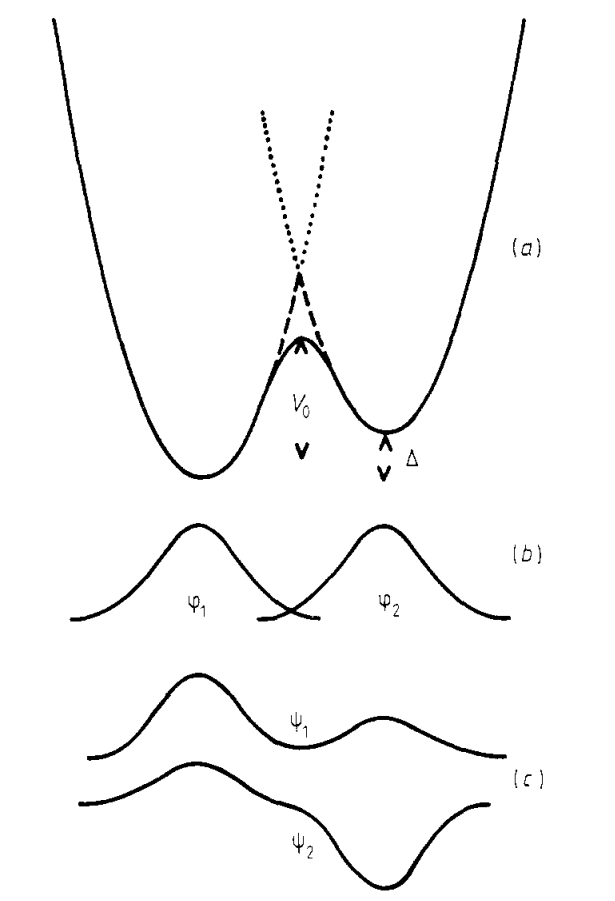
\includegraphics[width=0.4\textwidth]{CoupledPotentials.PNG}
		    \label{fig:CoupledPotentials}
      \end{figure}
     \end{block}
    \end{column}
		
    \begin{column}{.5\textwidth}
      \begin{block}{Coupled Hamiltonian}
       \scalemath{.6}{
        \begin{pmatrix}
          E_1 + <\phi_1|V-V_1|\phi_1> & <\phi_1|H|\phi_2> \\
          <\phi_2|H|\phi_1> & E_2 + <\phi_2|V-V_2|\phi_2>
         \end{pmatrix}}
      \end{block}
     \end{column}
		
\end{columns}
\end{frame}	
		

\begin{frame}[Early 00's]{First Ideas}

  \begin{itemize}
  \item
    Affect oscillation amplitude (Not $T_1$). 
  \item Early publications emphasized first measured single TLS-qubit interaction (not bulk).\textsuperscript{\cite{Simmonds}}
	\item {Theory (< 2004) concluded on current coupling. \textsuperscript{\cite{3}}}

  \end{itemize}

\end{frame}

\section{TLS Properties (and Applications?)}

\begin{frame}{TLS Properties}

  \begin{enumerate}
  \item Energy level repulsion.\textsuperscript{\cite{5}}
		\only<1>{\begin{figure}[htbp]
		    \centering
			  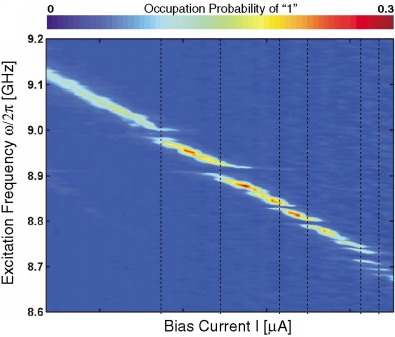
\includegraphics[width=0.6\textwidth]{TLS_Location_Spectroscopy.PNG}
		    \label{fig:TLS_Location_Spectroscopy}
      \end{figure}}
	\item \visible<2->{Warming a few Kelvin does not noticeably affect the system.}
	\item \visible<3->{Full warm-up and cool-down repopulates the system with TLS.}
  \item \visible<4->{TLS location in frequency can change spontaneously.}
  \end{enumerate}
\end{frame}


\begin{frame}{Storing Data in TLS}
In 2008, the Martinis Group (UCSB) coupled a phase qubit to a two-level system. They coherently swapped arbitrary states between the qubit and the two-level system with high fidelity (79\%).\textsuperscript{\cite{4}}
\\~\\
\ However, this is likely not to see further application (uncontrolled TLS location, other methods available, uncontrolled coupling strength, etc.)
\end{frame}

\section{Avoidance Techniques}

 \begin{frame}{Avoiding Them}
	\begin{itemize}
		\item
			Use Silicon-Nitride for junctions (not Si$0_2$)\textsuperscript{\cite{5}}
		  \only<1>{\begin{figure}[htbp]
		    \centering
			  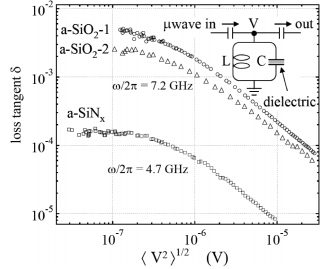
\includegraphics[width=0.6\textwidth]{MaterialsLossTangent.PNG}
		    \label{fig:Materials}
      \end{figure}}
		\item
			\visible<2->{Reduce junction size\textsuperscript{\cite{5}}}
			\only<2>{\begin{figure}[htbp]
		    \centering
			  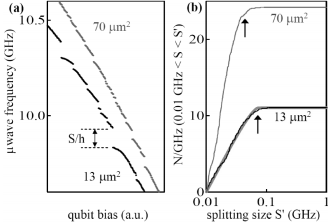
\includegraphics[width=0.6\textwidth]{JunctionSize.PNG}
		    \label{fig:JunctionSize}
				\end{figure}}
		\item
			\visible<3->{Use better resonator materials\textsuperscript{\cite{6}}}
			 \only<3>{\begin{figure}[htbp]
		    \centering
			  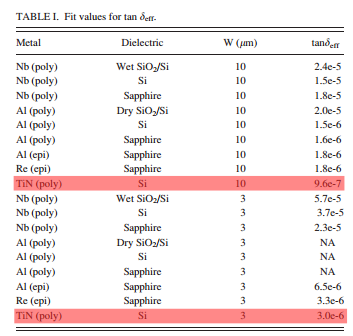
\includegraphics[width=0.5\textwidth]{LossTangents.PNG}
		    \label{fig:LossTangents}
				\end{figure}}
		\item
			\visible<4->{Use MBE deposition\textsuperscript{\cite{7}}}
			 \only<4>{\begin{figure}[htbp]
		    \centering
			  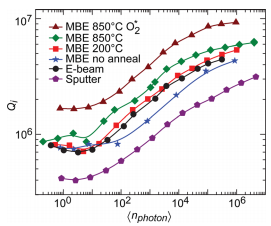
\includegraphics[width=0.6\textwidth]{DepTechs.PNG}
		    \label{fig:DepTechs}
				\end{figure}}				
	\end{itemize}
 \end{frame}

\begin{frame}[allowframebreaks]{References}
\begin{thebibliography}{9}
\setbeamertemplate{bibliography item}[text]
\bibitem{Phillips} Phillips, W. A. ``Two-level States in Glasses.'' Reports on Progress in Physics 50, no. 12 (1987): 1657.
\bibitem{Simmonds} Simmonds, R. W., K. M. Lang, D. A. Hite, S. Nam, D. P. Pappas, and John M. Martinis. ``Decoherence in Josephson Phase Qubits from Junction Resonators.''
\bibitem{3} Martinis, John M., K. B. Cooper, R. McDermott, Matthias Steffen, Markus Ansmann, K. D. Osborn, K. Cicak, et al.``Decoherence in Josephson Qubits from Dielectric Loss.'' Phys. Rev. Lett. 95, no. 21 (November 2005): 210503. doi:10.1103/PhysRevLett.95.210503.
\bibitem{4} Neeley, Matthew, M. Ansmann, Radoslaw C. Bialczak, M. Hofheinz, N. Katz, Erik Lucero, A. O Connell, H. Wang, A. N. Cleland, and John M. Martinis. ``Process Tomography of Quantum Memory in a Josephson-Phase Qubit Coupled to a Two-Level State.'' Nat Phys 4, no. 7 (July 2008): 523 - 526. doi:10.1038/nphys972.
\bibitem{5} Martinis, John M., K. B. Cooper, R. McDermott, Matthias Steffen, Markus Ansmann, K. D. Osborn, K. Cicak, et al. ``Decoherence in Josephson Qubits from Dielectric Loss.'' Phys. Rev. Lett. 95, no. 21 (November 2005): 210503. doi:10.1103/PhysRevLett.95.210503.
\bibitem{6} Sage, Jeremy M., Vladimir Bolkhovsky, William D. Oliver, Benjamin Turek, and Paul B. Welander. ``Study of Loss in Superconducting Coplanar Waveguide Resonators.'' Journal of Applied Physics 109, no. 6 (2011): 063915. doi:10.1063/1.3552890.
\bibitem{7} Megrant, A., C. Neill, R. Barends, B. Chiaro, Yu Chen, L. Feigl, J. Kelly, et al. ``Planar Superconducting Resonators with Internal Quality Factors above One Million.'' Applied Physics Letters 100, no. 11 (2012): 113510. doi:10.1063/1.3693409.


\end{thebibliography}

\end{frame}

\end{document}


